\documentclass[10pt]{article}
\usepackage{amsmath}
\usepackage{amsfonts}
\usepackage{graphicx}

\setlength{\oddsidemargin}{0pt}
\setlength{\evensidemargin}{0pt}
\setlength{\textwidth}{6.5in}
\setlength{\topmargin}{0in}
\setlength{\textheight}{8.5in}

\setlength{\parskip}{1pc}
\setlength{\parindent}{0pt}

\newcommand{\ans}[1]{\textbf{#1}}

\begin{document}

\section*{Short Answers}

\subsection*{RTT}

\begin{enumerate}
\item Questions on experiment a:

\begin{itemize}
\item What percentage of the websites do not respond to pings at all? What percentage have at least one failed ping?

20 percent of the sites do not respond to pings at all.
\\
27 percent of the sites have at least one failed ping

\item Using the plot functions and \texttt{rtt\_a\_agg.json}, please plot a CDF of the median RTT of the websites that respond to ping.

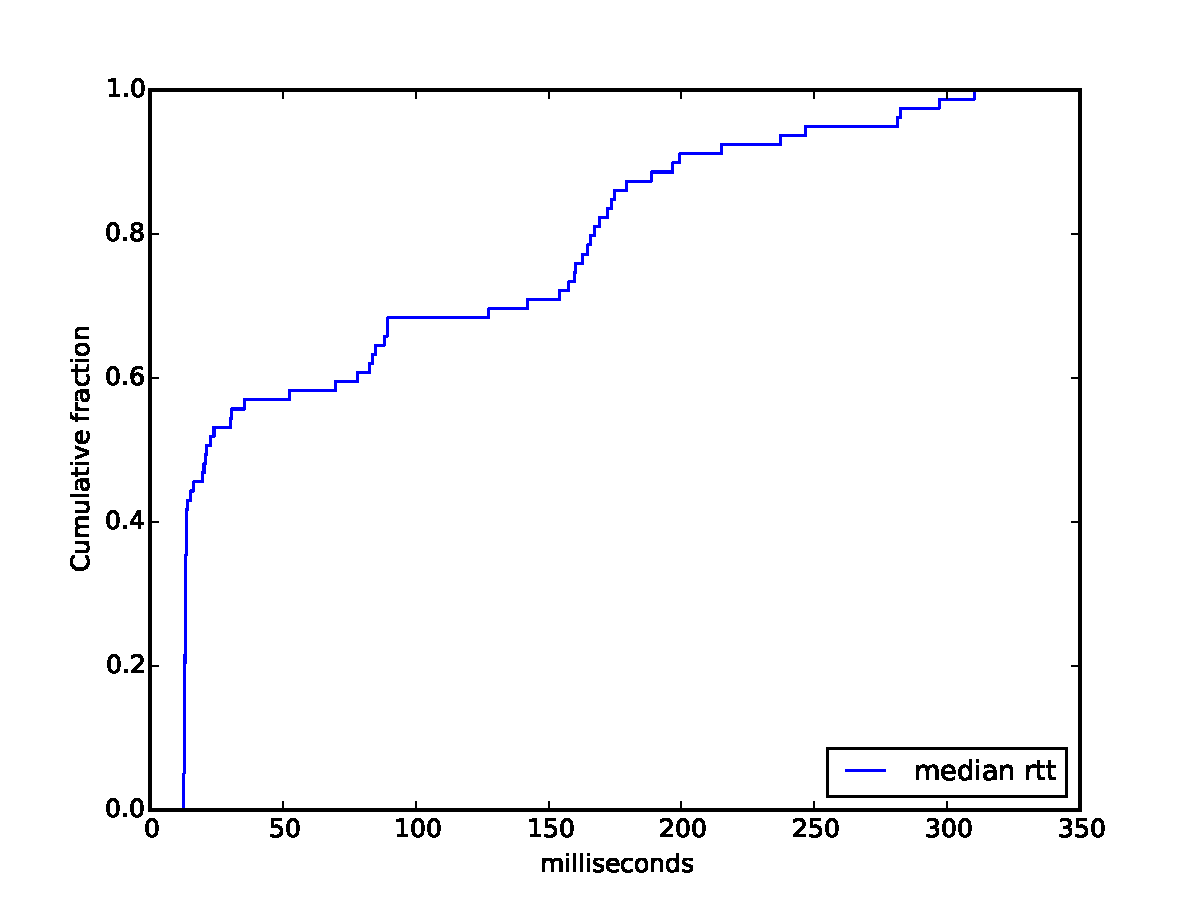
\includegraphics[scale=0.5]{plot_median_rtt.pdf}

\end{itemize}

\item Questions on experiment b:

\begin{itemize}

\item What are the median RTT and maximum RTT for each website? What loss rate do you observe?

todayhumor.co.kr \\
median rtt 13.235 \\
max rtt 97.743 \\
drop rate 0.0 \\
\\
google.com \\
median rtt 13.621 \\
max rtt 211.456 \\
drop rate 0.0 \\
\\
taobao.com \\
median rtt 293.772 \\
max rtt 512.706 \\
drop rate 2.800 \\
\\
zanvarsity.ac.tz \\
median rtt 391.846 \\
max rtt 526.934 \\
drop rate 2.400

\item Using the plot functions to and \texttt{rtt\_b\_raw.json}, please plot a CDF of the RTT for each website. You can plot the four CDFs on the same graph. Be sure to include a legend so we know which CDF corresponds to which of the four websites.

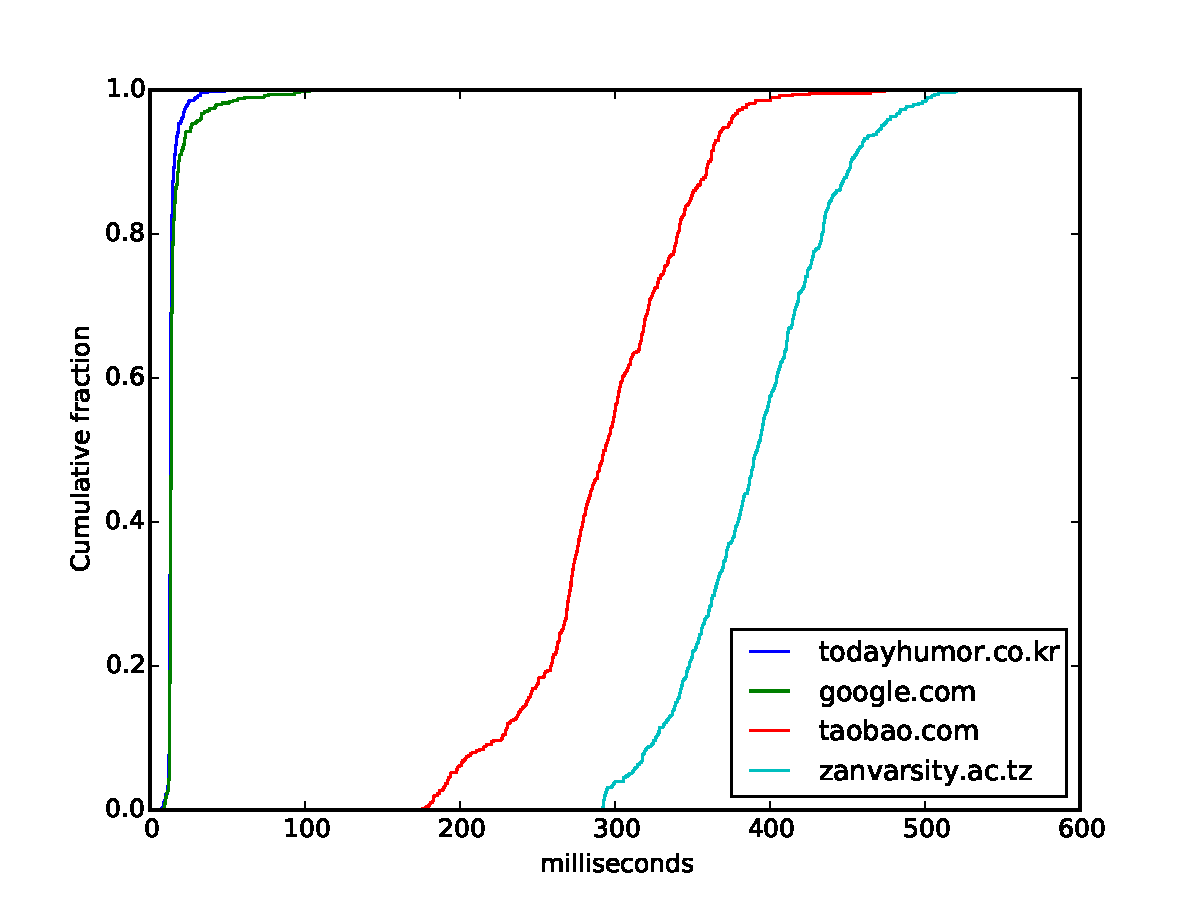
\includegraphics[scale=0.5]{plot_ping.pdf}

\end{itemize}

\item In this question, you will analyze the ping times to two websites and compare the results to the expected speed-of-light times. The websites are google.com (located in Mountain View, CA, USA) and zanvarsity.ac.tz (located in Zanzibar, Tanzania). You can use your ping data from experiment b. The distance from Berkeley to Mountain view is 35.23 miles, and the distance from Berkeley to Zanzibar is 9,953.50 miles.

\begin{itemize}

\item Compare the median ping time to the speed of light time. s the multiplier for each server (calculate as [ping time / speed of light time])?

google.com \\
median rtt = 13.621 ms \\
distance = 35.23 miles \\
speed of light = 186282 miles/second \\
speed of light rtt = ((35.23 * 2)/186282) s \\
speed of light rtt = 0.37824373798 ms \\
\\
(ping time / speed of light time) = 36.0111 \\

zanvarsity.ac.tz
median rtt = 391.846 ms \\
distance = 9,953.50 miles \\
speed of light = 186282 miles/second \\
speed of light rtt = ((9,953.50 * 2)/186282) s \\
speed of light rtt = 106.864860802 ms \\
\\
(ping time / speed of light time) = 3.6667

\item Using one sentence each, list two reasons why the ping time is not equal to the speed of light time. Plausible but unlikely answers (e.a bear chewed through the wire, causing a long delay) will not receive full credit.

1. The ping packet must go through various repeaters, switches and routers and each of these will slow down transfer speeds since they need time to process and route the ping packet.
\\
2. The ping packet will traverse most of its journey in fiber and data travels at roughly 2/3 the speed of light in fiber.


\item \emph{[Optional]} Repeat \#3 for any website you might be curious about. How much route inflation do you observe?

n/a

\end{itemize}
\end{enumerate}


\newpage
\subsection*{Routing}

\begin{enumerate}

\item Answer the following questions using the results obtained from experiment a

\begin{itemize}

\item Which ASes are Berkeley directly connected to?

25

\item Which traceroute traverses the most number of ASes? How about the least number of ASes?

Most : www.vutbr.cz, zanvarsity.ac.tz \\
Least : www.berkeley.edu

\item Which websites' routes are load-balanced?

google.com, facebook.com, allspice.lcs.mit.edu, todayhumor.co.kr, www.city.kobe.lg.jp, zanvarsity.ac.tz

\item Are the observed routes stable over multiple runs? For each website, how many unique routes did you observe?

google.com : Not Stable, 5 \\
facebook.com : Not Stable, 5 \\
www.berkeley.edu : Stable, 1 \\
allspice.lcs.mit.edu : Not Stable, 4 \\
todayhumor.co.kr : Not Stable, 5 \\
www.city.kobe.lg.jp : Not Stable, 5 \\
www.vutbr.cz : Stable, 1 \\
zanvarsity.ac.tz : Not Stable, 5

\item Using one sentence, please explain one advantage of having stable routes.

Stable routes are predictable and easy to debug. CHECK

\item \emph{[Optional]} Make a graph of the ASes and their connectivity.

n/a

\end{itemize}

\item Answer the following questions using the results obtained from experiment b.

\begin{itemize}

\item How many hops do you observe in each route when you run traceroute from your computer? How many hops do you observe in the reverse direction?

From public \\
tpr-route-server.saix.net : 13 \\
route-server.ip-plus.net : 12 \\
route-views.oregon-ix.net : 9 \\
route-views.on.bb.telus.com : 17 \\

To public \\
tpr-route-server.saix.net : 13 \\
route-server.ip-plus.net : 14 \\
route-views.oregon-ix.net : 8 \\
route-views.on.bb.telus.com : 10 \\

\item Are these routes symmetric? How many are symmetric and how many are not?

tpr-route-server.saix.net : Not symmetric \\
route-server.ip-plus.net : Not symmetric \\
route-views.oregon-ix.net : Not symmetric \\
route-views.on.bb.telus.com : Not symmetric \\
\\
0 are symmetric, 4 are not symmetric

\item What might cause asymmetric routes? List one or two reasons.

Asymmetric routes may be caused by load balancing. It could also be caused by ... CHECK

\end{itemize}
\end{enumerate}

\newpage
\subsection*{DNS}

\begin{enumerate}

\item What's the average root TTL in the 5 iterations of the top Alexa websites? Average TLD TTL? Average other name server TTL? Average terminating entry TTL?

Avg Root TTL : 431408.308 \\
Avg TLD TTL : 172800.0 \\
Avg Other NS TTL : 121008.152039555 \\
Avg Terminating TTL : 1018.1633663366337 \\

\item Plot a CDF of your 5 iterations from the Alexa top 100 websites using your \texttt{generate\_time\_cdfs} function (this should have two lines, as described above).

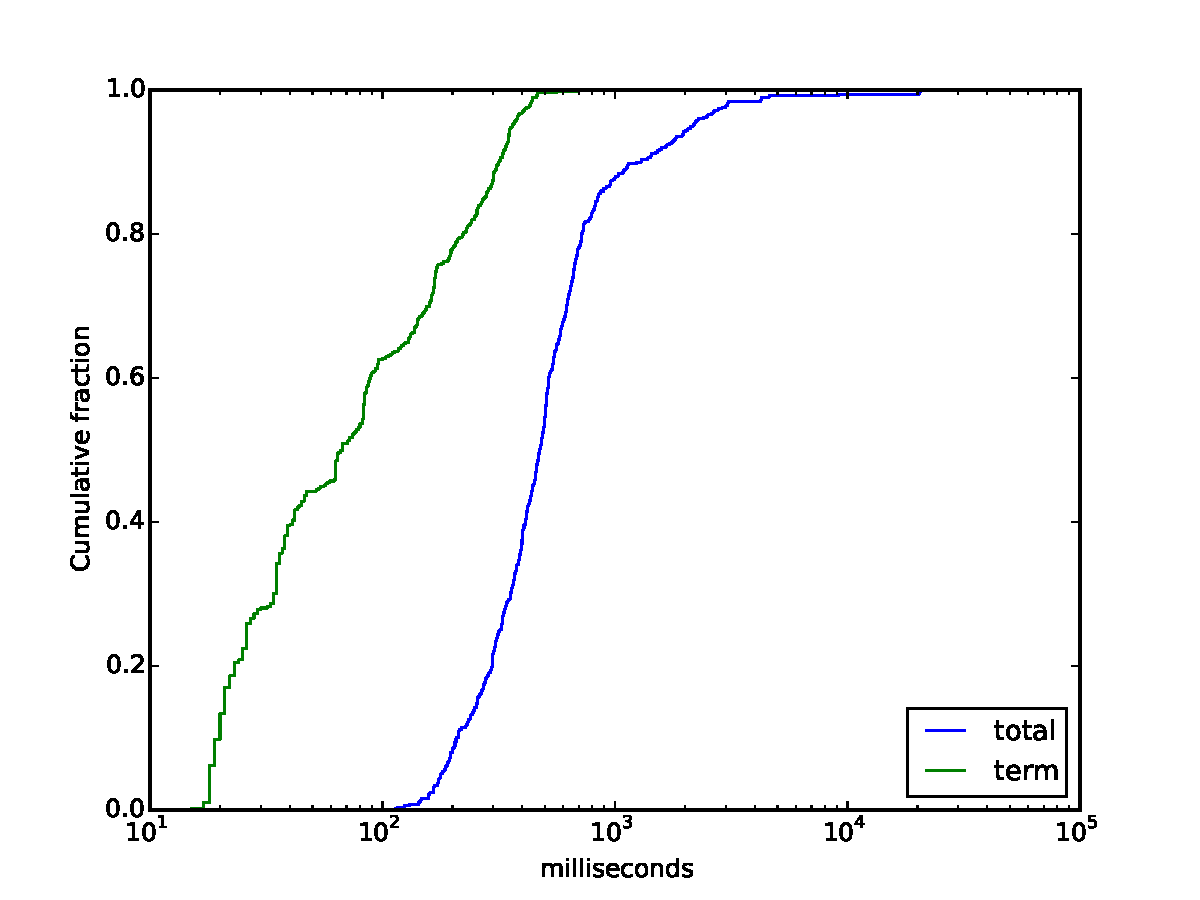
\includegraphics[scale=0.5]{plot_dig.pdf}

\item Run \texttt{run\_dig} twice at least 1 hour apart. How many answers change within the first trial? How many names gave different answers at some point in the two trials (i.e., what values does {count\_different\_dns\_responses} return?)?

7 changes in the First Trial and 10 changes between Both Trials

\item Run \texttt{run\_dig} using the name of a server in a different country. You can find public DNS servers in other countries here.
Run \texttt{count\_different\_dns\_responses} with your original trace and the one from the new country. What does it return?

7 changes in the First Trial and 31 changes between Both Trials

\item Take a look at a few of the names that returned different answers when you queried a different name server in the previous part. Use ping to measure the round trip time to the different IP addresses returned. What's the most likely reason that the different DNS server returned a different IP address? Answer in one sentence (you do not need to provide your ping output).

It could be that that the DNS servers are returning different IP addresses for load balancing purposes  CHECK

\item We asked you to use the \texttt{+trace} argument when running \texttt{dig}, which causes your local machine to resolve all requests iteratively starting from the root DNS server. How would the DNS resolution times have been different, and why if you hadn't used the \texttt{+trace} argument? Answer in 1 sentence.

Without using trace, the resolution times would be faster because it would not need to report the results from each query step.

\end{enumerate}

\end{document}